\documentclass[tikz,border=8pt]{standalone}
\usepackage{amsmath}
\usetikzlibrary{arrows.meta}

\begin{document}
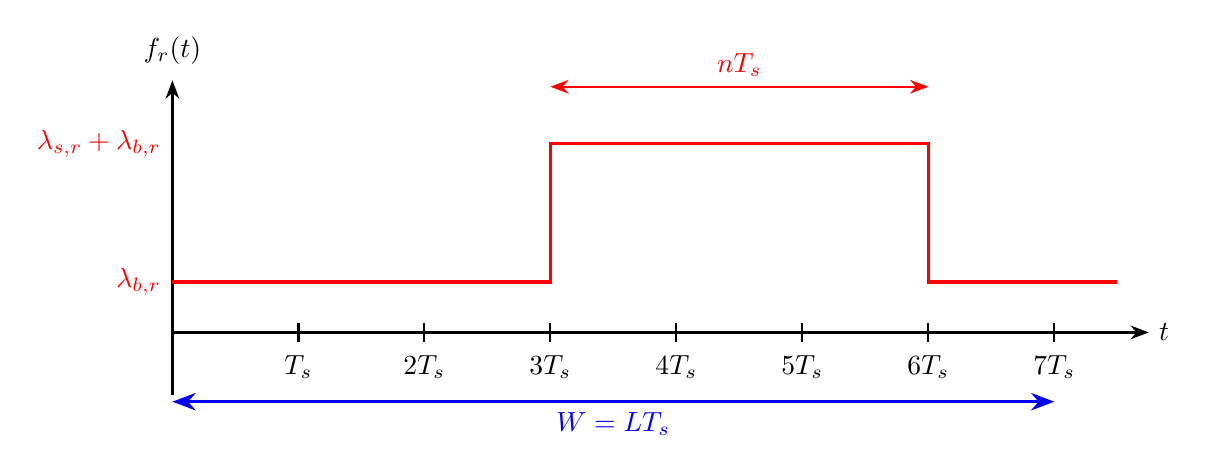
\begin{tikzpicture}[>=Stealth, thick, x=0.8cm, y=0.8cm]
  %--- parameters to tweak layout easily
  \def\xmin{0}
  \def\xmax{15}
  \def\ymin{-1.6}
  \def\ymax{4}
  \def\ybase{0.8}          % baseline level: \lambda_{b,r}
  \def\ytop{3.0}           % top level: \lambda_{s,r}+\lambda_{b,r}
  \def\apulse{6}           % pulse start x
  \def\bpulse{12}          % pulse end x
  \def\Ts{2}               % spacing for tick marks (visual only)

  %--- axes
  \draw[->] (\xmin,0) -- (\xmax+0.5,0) node[ right] {$t$};
  \draw[->] (0,\ymin+0.6) -- (0,\ymax) node[above=2pt] {$f_r(t)$};

  %--- red baseline + rectangular pulse
  \draw[very thick, red]
    (\xmin,\ybase) -- (\apulse,\ybase) --
    (\apulse,\ytop) -- (\bpulse,\ytop) --
    (\bpulse,\ybase) -- (\xmax,\ybase);

  %--- labels for levels
  \node[red, left=5pt] at (0.2,\ybase) {$\lambda_{b,r}$};
  \node[red, left=5pt] at (0.2,\ytop) {$\lambda_{s,r}+\lambda_{b,r}$};

  %--- nTs span over the pulse
  \draw[<->, red] (\apulse, \ytop+0.9) -- node[above, red] {$nT_s$} (\bpulse, \ytop+0.9);

  %--- tick marks every T_s (for look/feel)
\def\N{7} % number of ticks to draw
\foreach \i in {1,...,\N}{
  \pgfmathsetmacro{\x}{\i*\Ts}
  \draw (\x,0.15) -- (\x,-0.15);
  \node[below] at (\x,-0.2) {$\ifnum\i=1 T_s\else \i T_s\fi$};
}

  %--- long blue span W = L T_s
  \draw[<->, blue, very thick] (\xmin,\ymin+0.5) -- node[below, blue] {$W=L T_s$} (7*\Ts,\ymin+0.5);

\end{tikzpicture}
\end{document}
